\chapter{Computational Models for Encoding Natural Images}

\section{Introduction}
Sparse coding is a generative model for explaining natural signals. Although the model and motivating theory has been explored in other modalities, here we will focus on coding of images in the context of computation being performed by layer 4 cells in V1. We will begin this chapter with a probabilistic derivation for the sparse coding model. Importantly, this will make clear the various assumptions built into the model, which will be relevant for our interpretations of results in later chapters. The first section will get us to an energy function that a sparse coding algorithm would seek to minimize. The second section recapitulates the sparse coding model from an optimization perspective and outlines standard methods for inference and dictionary learning. Next, we will derive the Locally Competitive Algorithm, which is a neural network model designed to perform sparse inference. This network is the subject of the rest of the thesis. Finally, we will compare the LCA model to other popular neurally-inspired image coding models, namely Predictive Coding \parencite{rao1999predictive} and ICA \parencite{bell1997independent}.

\section{A probabilistic approach for image coding}
As was explained in chapter \ref{ch:intro}, the signal coming from the two-dimensional retinas is incomplete and the problem of inferring the exact three-dimensional structure of the world from that signal is impossible. However, some solutions are more likely than others and ecological pressure encourages brains to perceive highly likely solutions. If population activity in the brain represents possible hypotheses about the world, then we want to model it in a probabilistic, Bayesian framework. This section derives such a framework and shows that sparse coding approximately solves it.

We aim to encode an incoming signal efficiently under the assumption that the signal is composed of a structured component and unstructured additive noise. We do this with sparse coding, which assumes a linear generative model:

\begin{equation} \label{eq:ch2_generative_model}
    s = \Phi a + \varepsilon,
\end{equation}

\noindent where $s$ is our input signal, $\Phi$ is an overcomplete (in that the number of columns in $\Phi$ is greater than the number of rows) dictionary of functions, $a$ is a row vector of activation coefficients, and $\varepsilon$ is Gaussian noise. For a given input signal, we must solve the ill-posed task of inferring an optimal set of coefficients. The problem is difficult in part because the noise is unknown and therefore cannot be completely accounted for. Another reason is that the dictionary is overcomplete and thus non-orthogonal, resulting in an infinite number of possible combinations that are each equally valid representations. Following the works of Olshausen and colleagues \parencite{olshausen1996learning, olshausen2003principles, karklin1999porbabilistic}, we will derive a probabilistic generative model for computing image codes. Additionally, we can follow a similar derivation to learn a dictionary that maximize coding efficiency. This gives us a principled and extendable foundation from which we can derive sparse coding and similar models.

Our model assumes a prior probability over the images, $P(s)$, and the activity coefficients, $P(a)$. We also assume that the coefficient prior does not depend on the dictionary itself, that is $P(a|\Phi) = P(a)$. Although in practice the coefficients and dictionary will be jointly optimized, we can adhere to this last assumption by fixing one variable while optimizing the other in an expectation-maximization like procedure. We specify the likelihood of an image under the model for a given state of coefficients as $P(s|a,\Phi)$. Conversely, given evidence in the form of an image sample, we can define the posterior as the conditional probability distribution of our coefficients given the image and model: $P(a|s,\Phi)$. Our goal is to maximize this posterior distribution, which gives us the most probable estimate of the coefficients. As is done in \parencite{karklin1999porbabilistic}, we can relate the likelihood and posterior using Bayes' rule:

\begin{equation}\label{eq:ch2_bayes}
    P(a|s,\Phi) \propto P(s|a,\Phi) P(a)
\end{equation}

We model the noise distribution as Gaussian, which we justify by assuming that the generative model can account for everything except for random, uncorrelated (i.e. independent) causes that combine in the limit to follow a Gaussian distribution. Under this assumption, we can specify the probability density function for our image likelihood:

\begin{equation}\label{eq:ch2_image_likelihood}
    P(s|a,\Phi) \propto e^{-\frac{1}{2\sigma_{i}^{2}}|s-\phi a|^{2}},
\end{equation}

\noindent where $\sigma$ is the standard deviation of the additive noise. Our goal is to encode the images as efficiently as possible. To do this, we impose a factorial (i.e. independent) prior on the coefficients that is highly peaked at 0, which encourages most of the neurons to be silent for any given input signal. If we assume that the mean of the image distribution exists at $\Phi a$, then the maximum entropy distribution (with infinite variance) is Laplacian, which specifies the probability density function for our coefficient prior:

%TODO: Should these be f(a), etc? this is the functional form of the PDF right? so f(x) instead of P(x)?
\begin{equation}\label{eq:ch2_coefficient_prior}
    P(a) \propto \prod_{i}\frac{1}{\lambda} e^{\frac{-|a_{i}|}{\lambda}},
\end{equation}

\noindent where $\lambda = \tfrac{1}{\sigma^{2}}$. Finally, because we are assuming the noise is Gaussian, we can impose an $L_{2}$ prior on the pixel dimension of the dictionary:

\begin{equation}\label{eq:ch2_dictionary_prior}
    P(\Phi_{i}) \propto \frac{1}{\sqrt{2\pi}\sigma^{2}}e^{\frac{-\sum_{j}|\Phi_{i,j}|^{2}}{\sigma^{2}}}.
\end{equation}

Now that we have densities for our probabilities, we can write down the log-likelihood of our model, which we will later define as the negative of the sparse coding energy function:

\begin{align}\label{eq:ch2_log_likelihood}
\begin{split}
    \mathcal{L} &= \log\left(P(s|a,\Phi)P(a)\right) \\
                &= \log{P(s|a,\Phi)} + \log{P(a}) \\
                &= -\frac{\lambda}{2}|s - \Phi a|^{2} - \sum_{i}|a_{i}|.
\end{split}
\end{align}

Note that in the final step we dropped a constant term that is equal to the number of neurons times $\lambda$. Ideally, we would like to maintain a distribution of probable coefficients for a given image and model. However, we will only store the most likely coefficients using a maximum a-posteriori (MAP) estimate, which we justify by assuming that the distribution is highly peaked and therefore the maximum of the distribution is the most probable and a decent estimate of the mean. To estimate the most likely coefficients we can maximize their posterior given the data and model by finding a minimum of the negative log-likelihood:

\begin{align}\label{eq:ch2_min_log_likelihood}
\begin{split}
    \max_{a} p(a|s,\Phi) &= \max_{a}\left[\log{P(s|a,\Phi)} + \log{P(a)}\right] \\
                         &= \min_{a}\frac{\lambda}{2}|s - \Phi a|^{2} + \sum_{i}|a_{i}|.
\end{split}
\end{align}

The probability of the image under the model, $P(s|\Phi)$ is obtained by marginalizing over the internal states:

\begin{equation}\label{eq:ch2_image_probability}
    P(s|\Phi) = \int\partial a P(s|a,\Phi) P(a)
\end{equation}

If we wish to find the optimal dictionary, then we would again want to maximize the log of equation \ref{eq:ch2_image_probability}. However, it is not tractable to integrate over the coefficients to find the marginals, so instead we use a MAP estimate. This is a fair estimate if the model is sure of the posterior, that is to say that $P(a|s,\Phi)$ truly follows a highly peaked distribution with heavy tails (i.e. that the distribution has high kurtosis). Given this assumption, we define the log of the probability of the image under the model:

\begin{equation}\label{eq:ch2_log_image_probability}
    \log{P(s|\Phi)} = \log{\int P(s|a,\Phi)P(a)\partial a},
\end{equation}

\noindent and take the gradient with respect to our weights to give us a weight update rule:

\begin{equation}\label{eq:ch2_probability_weight_update}
    \nabla_{\Phi} \log{P(s|\Phi)} = \left< \left[s - \Phi a\right]a^{\top}\right>_{P(a|s,\Phi)}.
\end{equation}

The expectation in equation \ref{eq:ch2_probability_weight_update} tells us that we must do inference under the posterior. As we will see in the following section, the learning and inference rules can be derived directly from the same energy function, which is the negative of equation \ref{eq:ch2_log_likelihood}. Then we will make a simple change to the inference rule to define the LCA model. Finally, we will verify some known properties of sparse coding on natural images and derive comparisons to other similar models.


\section{Sparse coding}
In practice, sparse coding on images involves the tasks of learning a dictionary from data and, given a dictionary, finding an optimal sparse code for an input signal. We define an optimal sparse code as one that gives the most faithful representation of the data using the fewest dictionary elements. The primary objective of sparse coding, as described in \parencite{olshausen1997sparse}, is to encode input data (e.g. an image of a natural scene) in a generative framework, such that the data can be reconstructed from the code. Typically, we want the encoding to be of a higher dimensionality than the input image; that is to say we want our dictionary to be overcomplete.

For an $N$-dimensional input signal (e.g. an $N$ pixel image), $s \in \mathbb{R}^{N}$, we want a dictionary of $M > N$ vectors, where each vector is of length $N$. The dictionary is a matrix $\Phi$ with dimensions $N \times M$. Each of the $M$ columns are dictionary elements, $\Phi_{i}, i \in \{1,...,M\}$, and each dictionary element has a corresponding coefficient, $a_{i}, i \in \{1,...,M\}$, that we can assemble into a vector of activations. Our goal is to minimize an energy function that requires both a faithful and efficient representation of the data, in that it reconstructs the data well with the fewest number of active elements. We can express this mathematically as

\begin{equation}\label{eq:ch2_sparse_energy}
    \argmin\limits_{a, \Phi}
        \left( E =
            \overbrace{ \tfrac{1}{2} \| s - \hat{s} \|_{2}^{2} }^\text{Preserve Information} +
        \overbrace{ \lambda \sum\limits_{i=1}^{M}C(a_{i}) }^\text{Limit Activations} \right),
\end{equation}

\noindent where $\hat{s} = \sum\limits_{i=1}^{M}\Phi_{i}a_{i}$ is the image reconstruction, $\argmin\limits_{a, \Phi}$ tells us that we want to minimize the energy with respect to both the activations and the dictionary, and $||\cdot||_2^2$ indicates the squared $l_2$ norm. In this energy function, we use $\lambda$ as a trade-off penalty between the reconstruction quality and the sparsity constraint. Note that we have performed a change of variables from the previous section, to include the noise variance, $\sigma$ into a new $\lambda$ parameter that now modulates the $L_{1}$ cost as a Lagrange multiplier. In practice we tune it to maximize network sparsity for a minimum accepted reconstruction quality. One popular choice for the cost function, $C(\cdot)$, is the $l_1$ cost penalty, which is the sum of the absolute value of all activations:

\begin{align}\label{eq:ch2_l1_cost}
\begin{split}
  &C(a_{i}) = |a_{i}| \\
  &\sum\limits_{i=1}^{M}C(a_{i}) = \sum\limits_{i=1}^{M}|a_{i}|.
\end{split}
\end{align}

Depending on the choice of cost function, solving equation \eqref{eq:ch2_sparse_energy} can be convex or non-convex. For the $l_{1}$ cost, it is non-convex. Previous work has solved this via alternating projected gradient descent \parencite{olshausen1997sparse}, basis pursuit denoising \parencite{chen2001atomic}, or matching pursuit \parencite{davis1997adaptive, rehn2007network, rebollo2002optimized}. The basis pursuit denoising variant is often accomplished using the iterative shrinkage and thresholding algorithm (ISTA) \parencite{daubechies2004iterative, beck2009fast}. Rozell et al. \citeyearpar{rozell2008sparse} proposed an alternative to ISTA using a neural network following dynamics governed by the energy gradient. The following section explains this alternative in detail.


\section{The Locally Competitive Algorithm}\label{sec:ch2_lca}
The Locally Competitive Algorithm (LCA) is a method for computing a sparse code from a given input signal and dictionary and was original described by Christopher J. Rozell and colleagues \citeyearpar{rozell2008sparse}. The model describes an activation coefficient, $a_{k}$, as the thresholded output of some model neuron's internal state, $u_{k}$, which is analogous to the neuron's membrane potential. This internal state follows similar dynamics to a leaky integrator neuron model. The LCA can be described as a continuous system that is implementable in hardware, or as a discrete system with an internal state that advances as a function of a time step. If implemented in hardware, you can follow current dynamics (Kirchhoff's law for an equivalent RC circuit) to perform inference extremely quickly \parencite{rozell2008sparse}. As the model state advances, the system relaxes to a minimum solution of the energy function described in equation \eqref{eq:ch2_sparse_energy}. Here we will derive the dynamical equation for computing the state transitions from the energy function.

We wish for our neuron activations to minimize the energy function described in equation \eqref{eq:ch2_sparse_energy}. This will be accomplished via gradient descent on the energy function. To illustrate the derivative, we first express the energy function in subscript notation:

\begin{equation}\label{eq:ch2_subscript_sparse_energy_func}
    E(t) = \tfrac{1}{2} \sum\limits_{i=1}^{N} \left[ s_{i} - \sum\limits_{j=1}^{M}a_{j}(t) \Phi_{i,j} \right]^{2} + \lambda \sum\limits_{j=1}^{M} C(a_{j}(t))
\end{equation}

and then we take the derivative with respect to an individual neuron's activity, $a_{k}(t)$. Since we ultimately want to do gradient \textit{descent}, we will write the negative derivative:

\begin{align}\label{eq:ch2_lca_deda_extended}
\begin{split}
    - \frac{\partial E(t)}{\partial a_{k}(t)}
    =
        &\sum\limits_{i=1}^{N} S_{i} \Phi_{i,k} -
        \Phi_{i,k}\sum\limits_{j=1}^{M}a_{j}(t) \Phi_{i,j} -
        \lambda \sum\limits_{j=1}^{M}\frac{\partial C(a_{j}(t))}{\partial a_{k}(t)} \\
    =
        &\sum\limits_{i=1}^{N} \left[ s_{i} \Phi_{i,k} -
        \sum\limits_{j \neq k}^{M} \Phi_{i,k} \Phi_{i,j} a_{j}(t) - \Phi_{i,k}\Phi_{i,k}a_{k}(t) \right] -
        \lambda \frac{\partial C(a_{k}(t))}{\partial a_{k}(t)}
\end{split}
\end{align}

One constraint that we impose on our model is that we want the dictionary elements to all be unit norm in the pixel dimension, $||\phi_{i}||_2^2 = 1$. This means that the $\sum_{i=1}^{N}\Phi_{i,k}\Phi_{i,k}a_{k}(t)$ term in equation \eqref{eq:ch2_lca_deda_extended} reduces to $a_k(t)$:

\begin{equation}\label{eq:ch2_lca_deda}
    -\frac{\partial E(t)}{\partial a_{k}(t)} =
    \sum\limits_{i=1}^{N} \left[ s_{i} \Phi_{i,k} -
    \sum\limits_{j \neq k}^{M} \Phi_{i,k} \Phi_{i,j} a_{j}(t) \right] - a_{k}(t) -
    \lambda \frac{\partial C(a_{k}(t))}{\partial a_{k}(t)}
\end{equation}

Note that $E(t)$ and $a(t)$ both vary in time. In this scenario, we can imagine a constant input signal, $s$, and a constant set of dictionary elements, $\Phi$. Given these constants, we want the system to evolve over time to produce an optimal set of activations, $a$. Equation \eqref{eq:ch2_subscript_sparse_energy_func} gives us the energy at each time point during this inference process. Each neuron has a corresponding dictionary element, $\phi_{k}$, which is a vector that indicates the connection strength to each pixel in the input. In the literature this is also referred to as the strength of the synaptic connections between the neuron and each input pixel, or the neuron's feed-forward receptive field. In this model, we are going to find a sparse code for each individual image patch, so all $M$ neurons will be connected to the same image patch, $s$. The model neuron has a driving excitatory input, which we will denote $b_{k} = S\phi_{k} = \sum_{i=1}^{N}s_{i} \Phi_{i,k}$. This is the projection of the input image onto the neuron's corresponding dictionary element. The stronger the similarity between the input, $s$, and the dictionary element, $\phi_{k}$, the stronger the driving excitatory input. Each neuron also receives inhibition from every other active neuron. The magnitude of inhibition is partially set by an $M \times M$ Gramian matrix, $G$. The matrix evaluates to the inner product of the each neuron's dictionary element with all other neurons' dictionary elements, $G = \Phi^T\Phi$, such that each element in $G$ gives the overlap in pixel space between two dictionary elements, $G_{i,j} = \sum\limits_{n=1}^{N} \Phi_{n,i}\Phi_{n,j}$. The total inhibition onto a neuron is also scaled by how active the inhibiting neuron is.

Next, we define a new function that maps the activity for a neuron and the sparsity cost function to a new scalar. This function can be thought of as the self inhibition that increases as the value of $a_{k}$ increases:

\begin{equation}\label{eq:ch2_hopfield_t_func}
  f_{\lambda}(a_{k}(t)) = a_{k}(t) + \lambda \frac{\partial C(a_{k}(t))}{\partial a_{k}(t)}
\end{equation}

Now we can write the partial derivative of our energy function (equation \eqref{eq:ch2_subscript_sparse_energy_func}) in terms of our new variables:

\begin{equation}\label{eq:ch2_lca_deda_simple}
    - \frac{\partial E(t)}{\partial a_{k}(t)} =
    b_{k} -
    \sum\limits_{j \neq k}^{M} G_{k,j} a_{j}(t) -
    f_{\lambda}(a_{k}(t)).
\end{equation}

At this point we could update $a(t)$ using gradient descent following equation \eqref{eq:ch2_lca_deda_simple} to produce a sparse code from an input signal. A more biologically consistent solution would be to have the model neuron maintain an internal state, analogous to a biological neuron's membrane potential. The model neuron could then only produce output when its membrane potential passed over some threshold. This will have better correspondence to biology and it will give the neurons sub-threshold dynamics that will influence their activity (see section \ref{sec:ch2_lca_properties}) when compared to directly using equation \ref{eq:ch2_lca_deda_simple}. Following this logic, Rozell et al. \citeyearpar{rozell2008sparse} define an internal state variable, $u_{k}(t)$ that represents the membrane potential for neuron $k$ at time $t$. When a neuron's potential climbs above some threshold, it communicates in the form of an activation, $a_{k}(t)$, which is analagous to a spike rate. Only these excited neurons can contribute to the image code and reconstruction. Ultimately, the network of neurons should still descend the energy function from equation \eqref{eq:ch2_subscript_sparse_energy_func}, so we define the neuron's state dynamics to be governed by the following equation:

\begin{align}\label{eq:ch2_u_dot}
\begin{split}
    \dot{u_{k}}(t) &\propto - \frac{\partial E(t)} {\partial a_{k}(t)} \\
    \dot{u_{k}}(t) &= \frac{1}{\tau} \left[b_{k} - \sum_{m \neq k}^{M}G_{k,m}a_{m}(t) - f_{\lambda}(a_{k}(t)) \right],
\end{split}
\end{align}

\noindent where $\tau$ is a proportionality constant that represents the time constant of the dynamics.

In order to have a complete description of the model, we need to describe a relationship between $u$ and $a$. Earlier the $f_{\lambda}(a_{k}(t))$ term was described as a self inhibition term that encourages sparsity. Another way to enforce self inhibition is to introduce a membrane leak term. If we assign the internal state, $u_{k}(t)$, to this function:

\begin{equation}\label{eq:ch2_u_func_a}
    u_k(t) = f_{\lambda}(a_{k}(t)),
\end{equation}

\noindent then we can think of our neuron as a leaky integrator. We can also invert the function to get our neuron's output activity:

\begin{displaymath}\label{eq:ch2_a_fu_thresh}
    a_{k}(t) = f_{\lambda}^{-1}(u_{k}(t)) := T_{\lambda}(u_{k}(t)).
\end{displaymath}

This gives us the LCA neuron update equation:
\begin{equation}\label{eq:ch2_u_dot_full}
    \dot{u_{k}}(t) = \frac{1}{\tau} \left[\overbrace{b_{k}}^\text{Driving excitation} - \overbrace{\sum_{m \neq k}^{M}G_{k,m}a_{m}(t)}^\text{Lateral Inhibition} - \overbrace{u_{k}(t)}^\text{Leak} \right],
\end{equation}

\noindent or equivalently:

\begin{displaymath}
    \tau \dot{u_{k}}(t) + u_{k}(t) =  b_{k} - \sum_{m \neq k}^{M}G_{k,m}a_{m}(t).
\end{displaymath}

When the neuron's membrane potential passes over a threshold, defined by $T_{\lambda}(u_{k}(t)) = f_{\lambda}^{-1}(u_{k})$, it becomes active:

\begin{equation}\label{eq:ch2_a_thresh}
  a_{k}(t) = T_{\lambda}(u_{k}(t))
\end{equation}

For this expression to perform gradient descent on the energy function, $a$ must be a monotonically increasing function of $u$. Rozell et al. \citeyearpar{rozell2008sparse} describe the relationship between the sparseness cost penalty, the neuron activity, and the internal membrane potential via a thresholding function. The thresholding function can take various forms that determine the exact nature of the sparseness penalty. For the $l_{1}$ penalty, we use a soft thresholding function:

\begin{equation}\label{eq:ch2_lca_threshold_func}
    T_{\lambda}(u_{k}(t)) = \left\{
    \begin{aligned}
        u_{k}(t)+\lambda,\;\; &u_{k}(t)\; <\; -\lambda \\
        0,\;\; &-\lambda < u_{k}(t)\; <\; \lambda \\
        u_{k}(t)-\lambda,\;\; &u_{k}(t)\; >\; \lambda
    \end{aligned}
    \right.
\end{equation}

Here $\lambda$ indicates the sparseness penalty trade-off as well as the threshold that the membrane potential must surpass for the neuron to become active. An illustration of how one gets to the thresholding function from the $l_{1}$ penalty is given in figure \ref{fig:ch2_lca_thresh}. With the internal state dynamics from equation \eqref{eq:ch2_u_dot_full} and the thresholding function in equation \eqref{eq:ch2_lca_threshold_func}, we have defined a network that settles to a sparse code, $a$, that represents the input signal. For all of the work in this thesis, we will diverge from the implementation in \parencite{rozell2008sparse} and implement a rectified version of the thresholding function. That is, from equation \ref{eq:ch2_lca_threshold_func}, the last term for when $u_{k}(t) > \lambda$ is set to $T_{\lambda}(u_{k}(t))=0$. This adds a higher degree of nonlinearity, and is important for implementing hierarchical sparse coding models.

\begin{figure}[h]\label{fig:ch2_lca_thresh}
\centering %center using container as reference, instead of the whole text
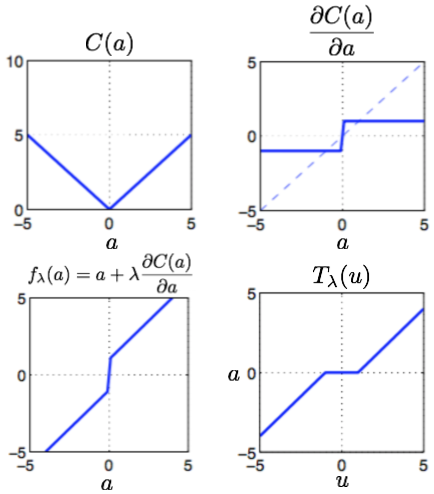
\includegraphics[width=0.5\textwidth]{lca_cost_graphs.png}
\caption{\textbf{Deriving the LCA thresholding function} Starting from a pictorial view of the $l_{1}$ cost function, one can derive the self inhibition term from equation \eqref{eq:ch2_u_func_a} and invert it to see the thresholding function described in equation \eqref{eq:ch2_lca_threshold_func}. Notice that the value of $\lambda$ dictates the range of allowable sub-threshold membrane potentials, $u_{k}$, before the neuron becomes active.}
\end{figure}

In addition to finding a sparse code, we are also interested in learning a set of dictionary elements, $\Phi$. This can be done by performing gradient descent on equation \eqref{eq:ch2_sparse_energy} using the coefficient values obtained with LCA. This yields

\begin{equation}\label{eq:ch2_phi_update}
    \Delta \phi_{k} = \eta (s - \hat{s}) a_{k},
\end{equation}

\noindent where $\eta$ is the learning rate and $\hat{s}$ is the image reconstruction. To recap, for a given image sample we first find our image code, $a$, for a fixed dictionary, $\Phi$, and then using that code to update the dictionary with equation \eqref{eq:ch2_phi_update}.


\subsection{Convolutional LCA}
In this thesis, unless otherwise noted, it should be assumed that we are using the traditional, fully-connected variant of LCA.

LCA can be easily extended to a convolutional variant. In previous sections, we described the model as being \textit{fully connected}, in that each neuron was connected to every pixel in the input, which was defined as square image patches with typically around 12 pixels on a side. To scale this up to larger images we can redefine LCA as convolutional. There are benefits to convolutional over fully-connected LCA: it is more amenable GPU architectures, it converges to lower minima, and it is more stable when encoding video. However, downsides are that it no longer has a straight forward analog hardware implementation and it diverges from the type of connectivity we see in the brain. A possible better alternative to convolution would be to use local (i.e. tiled) connectivity, as was done in \parencite{le2011building} and \parencite{ngiam2010tiled}. At the time of writing we are unaware of any attempt to use this type of connectivity with LCA.

In future chapters we will occasionally use convolutional LCA to scale up experiments to larger inputs. For a neural-network oriented introduction to convolution, see \parencite{goodfellow2019deep}. The convolution will be parameterized by a kernel size, number of kernels, and stride. If the stride is equal to the patch size (i.e. no overlap), then this model implements regular patch-based LCA that operates on an entire image worth of patches as a batch. To do this, we write our energy function in terms of a ``deconvolution'', or transposed convolution \cite{zeiler2010deconvolutional}:

\begin{equation}
    E = \frac{1}{2} || s - a \circledast \Phi ||^{2}_{2} + \lambda ||a||_{1},
\end{equation}

\noindent where $\circledast$ is the transposed convolution operator. We also rewrite the membrane update equation to be in terms of a residual error convolved with the weight vector:

\begin{equation}\label{eq:ch2_conv_lca_dynamics}
   \tau \dot{u_{k}} + u_{k} = e \ast \Phi_{k} + a_{k},
\end{equation}

\noindent where $\ast$ is convolution and $e = s - \hat{s}$ is the residual error. In this variant, the driving force to the neurons is the error, instead of the $b_{k}$ term in equation \ref{eq:ch2_lca_deda_simple}. This means that every neuron that is competing for the image reconstruction will contribute to driving neuron $k$, even if it is in a different convolutional position. The effects of this global competition across the image appear to give the model an advantage in terms of finding an energy minima and stability, which we demonstrate in figure \ref{fig:ch2_lca_conv_benefit}.

\begin{figure}[h]\label{fig:ch2_lca_conv_benefit}
    \centering
    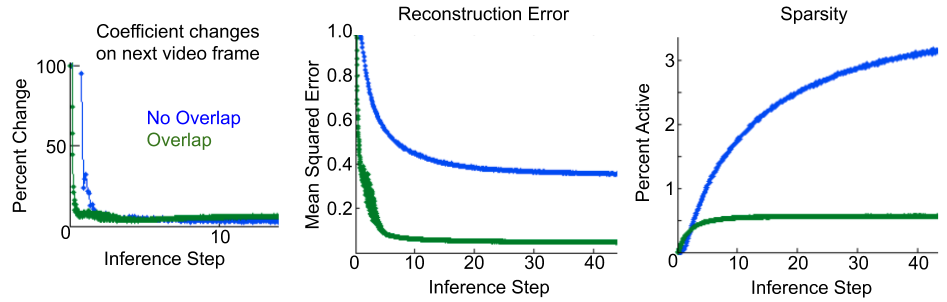
\includegraphics[width=\textwidth]{figures/lca_conv_benefits.png}
    \caption{Convolutional LCA (overlap, green lines) has better encoding properties than patch-based LCA (no overlap, blue lines). This is likely an effect of global competition across the image that is afforded by the convolutional architecture. Note that the patch-based LCA is still sharing weights between patches; it is acting as if each patch was encoded independently with the same model. Left - For video input, we recorded the percent change in coefficients from one frame to the next as a function of the number of inference steps allowed on each frame. The convolutional variant is more stable earlier in inference, and equally stable after both variants have converged. Middle - Convolutional LCA settles to a lower mean squared error than the patch-based model. Right - Convolutional LCA is more sparse than the patch-based model. This figure was reproduced from unpublished work done with the Kenyon lab \citeyearpar{paiton2013deep}.}
\end{figure}


\subsubsection{A note on overcompleteness}
In patch-based sparse coding, we compute the network overcompleteness by dividing the number of neurons by the number of pixels. However, with convolutional sparse coding there is a caveat that the neighboring inputs have shared weights. Therefore, directly expressing the overcompleteness as number of outputs / number of inputs misrepresents the number of unique weights in the model. Even more nuanced is that LCA typically learns weights that tile all possible positions in the image patch, which is not as necessary with a convolutional model since the convolution operation translates weights across the image. As a result, all weights learned with convolution tend to be centered in their patch. With all of this in mind, we will denote convolutional overcompleteness as the number of kernels divided by the product of the x and y strides: $o = \tfrac{f}{s_{x}*s_{y}}$. Therefore, within reasonable parameter ranges, you can effectively increase the overcompleteness by increasing the number of kernels or by decreasing the stride, which important when considering computational constraints \parencite{schultz2014replicating}. From this we can also conclude that overcompleteness is not dependent on the size of the patch size, which has been exploited for learning disparity selective neurons that require large receptive fields \parencite{lundquist2016sparse}.


\subsection{Postdictions from the LCA}
In their landmark paper, Olshausen and Field \citeyearpar{olshausen1996emergence} show that the sparse coding model learns oriented, band-pass receptive fields. These are well matched to fits of the linear approximations of receptive fields of mammalian V1 simple cells obtained via spike-triggered averaging \parencite{vanHateren1998independent}. They argue that this supports the hypothesis that the V1 neural population encodes visual stimulus using an efficient wavelet-like dictionary. This result has been replicated a number of times with various types of sparse coding models \citeyarpar{zylberberg2011sparse, zylberberg2013sparse, rehn2007network}. As a followup to this study, \parencite{zhu2013visual} show that the LCA network also exhibits a variety of extra-classical receptive field effects, including end-stopping, cross-orientation inhibition, and surround suppression. This is an important finding, as it shows that a single LCA network trained on natural scenes matches well the linear and non-linear empirical effects found with biological neurons. Most studies of these non-linear effects employ unique models that are extended from the classic linear/non-linear neuron model (see section \ref{sec:ch2_alternative_image_coding_models}) for each effect found, while Zhu and Rozell are able to demonstrate many effects with a single model. In Chapter \ref{ch:iso} we will argue that these effects result from the explaining away process during sparse inference. In \citeyearpar{vinje2000sparse}, the authors find that stimulating the nCRF (non-classical receptive field) with naturalistic stimuli causes pairs of V1 neurons to become more decorrelated in their response. They observed ``dramatically increased sparseness'' when stimulating nCRFs, and suggest that a consequence of this ``is increased independence of the responses across cells''. note haider et al work and adesnik work.

As we will expand on in chapter \ref{ch:iso}, the LCA makes explicit predictions about the existence (and necessity) of population non-linearities among V1 neurons, which facilitate unique responses to natural image stimuli. In addition to the obvious energy saving motivation for sparse activity, it has been argued that limiting the number of active neurons can result in a more explicit code that is easier to read out by downstream neurons \parencite{olshasen2002principles}. We will explore this in more detail in chapters \ref{ch:iso} and \ref{ch:semi-supervised}.

\section{Properties of LCA trained on natural images}\label{sec:ch2_lca_properties}
\subsection{Features learned}
It has been shown previously that sparse coding will learn a dictionary of features that tile spatial position, frequency, and orientation \cite{olshausen1996emergence, olshausen1997sparse}. Here we reproduce this finding while also varying the overcompleteness of the model in figure \ref{fig:ch2_lca_overcompleteness_tiling}. We find that as overcompleteness increases, the density of the tiling also increases. Additionally, the model learns higher spatial frequency features and a more even distribution of orientations when more overcomplete. It is also interesting that the models tend to learn significantly more features that are aligned with the vertical and horizontal axis of the input images, which is well matched to image statistics \parencite{switkes1978spatial, torralba2003statistics}.

\begin{figure}[h]\label{fig:ch2_lca_overcompleteness_tiling}
    \centering
    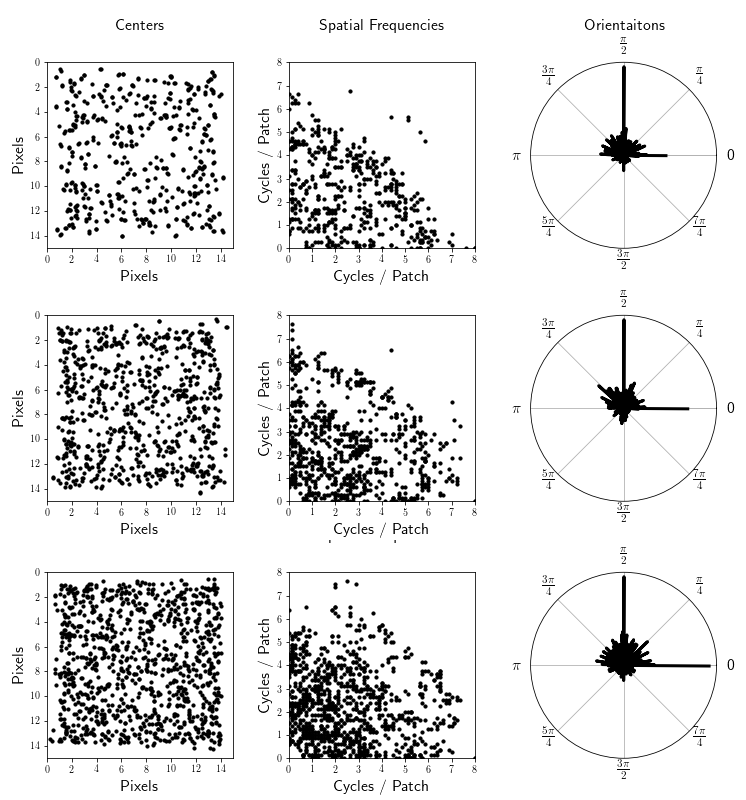
\includegraphics[width=\textwidth]{figures/lca_overcompleteness_location_frequency_centers.png}
    \caption{LCA learns a feature set that tiles spatial positions, frequencies, scales, and orientations when trained on natural scenes. Here we demonstrate this while also varying overcompleteness. Each column is a level of overcompleteness for LCA trained on 16 by 16 pixel Fourier whitened \ref{sec:appendix_preprocessing} image patches. The columns each represent LCA with 2, 3, and 4 times more neurons from the top to bottom, respectively. The rows from left to right are the spatial positions, spatial frequency, and orientation of each function.}
\end{figure}

\subsection{Inferring sparse codes of natural images with LCA}
Inference is a critical component of the sparse coding model. It gives the model the ability to ``explain away'' causes of the input signals \parencite{olshausen1997sparse} and gives neurons a higher degree of selectivity (see chapter \ref{ch:iso}). Figure \ref{fig:ch2_lca_inference_loss} shows the values of the loss function in equation \ref{eq:ch2_sparse_energy} through inference, demonstrating that the total loss is reduced. Notice that the sparse loss starts at zero, indicating that none of the neurons are contributing to the reconstruction. At the beginning of inference, all of the neurons with a non-zero inner product with the input have an increase in membrane potential without any inhibition from other neurons. It is only after a neuron passes threshold that it starts inhibiting its neighbors. These sub-threshold dynamics can result in a better solution than the standard ISTA framework, which turns on all units with a non-zero inner product with the input at the first inference step \cite{rozell2008sparse}.

\begin{figure}[h]\label{fig:ch2_lca_inference_loss}
    \centering
    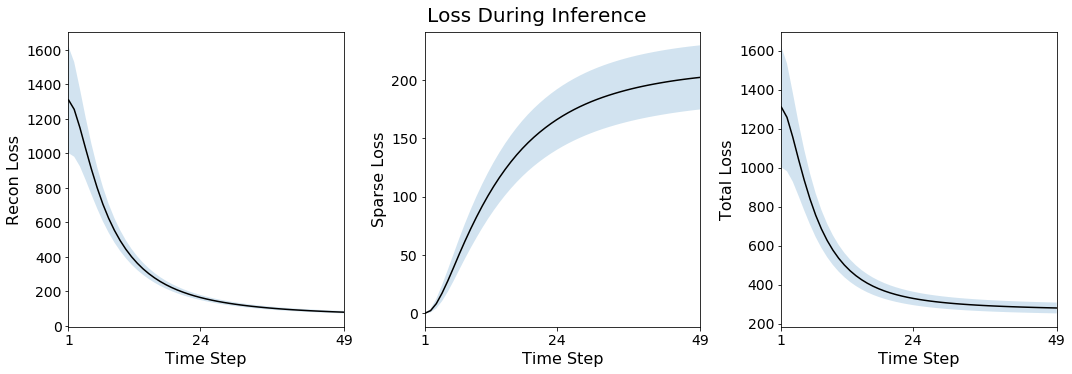
\includegraphics[width=\textwidth]{figures/lca_inference_loss.png}
    \caption{LCA inference minimizes the sparse coding energy function (equation \ref{eq:ch2_sparse_energy}). Black lines represent the mean of 50 natural scenes and the blue background represents the standard error of the mean.}
\end{figure}

Figure \ref{fig:ch2_lca_inference_traces} gives us an idea of the inference dynamics for the a subset of neurons in the LCA network. Each line in the trace plots represents a different term from equation \ref{eq:ch2_lca_deda_simple}. Nearly all of the traces follow nonlinear trajectories, and have interesting sub-threshold dynamics.

\begin{figure}[h]\label{fig:ch2_lca_inference_traces}
    \centering
    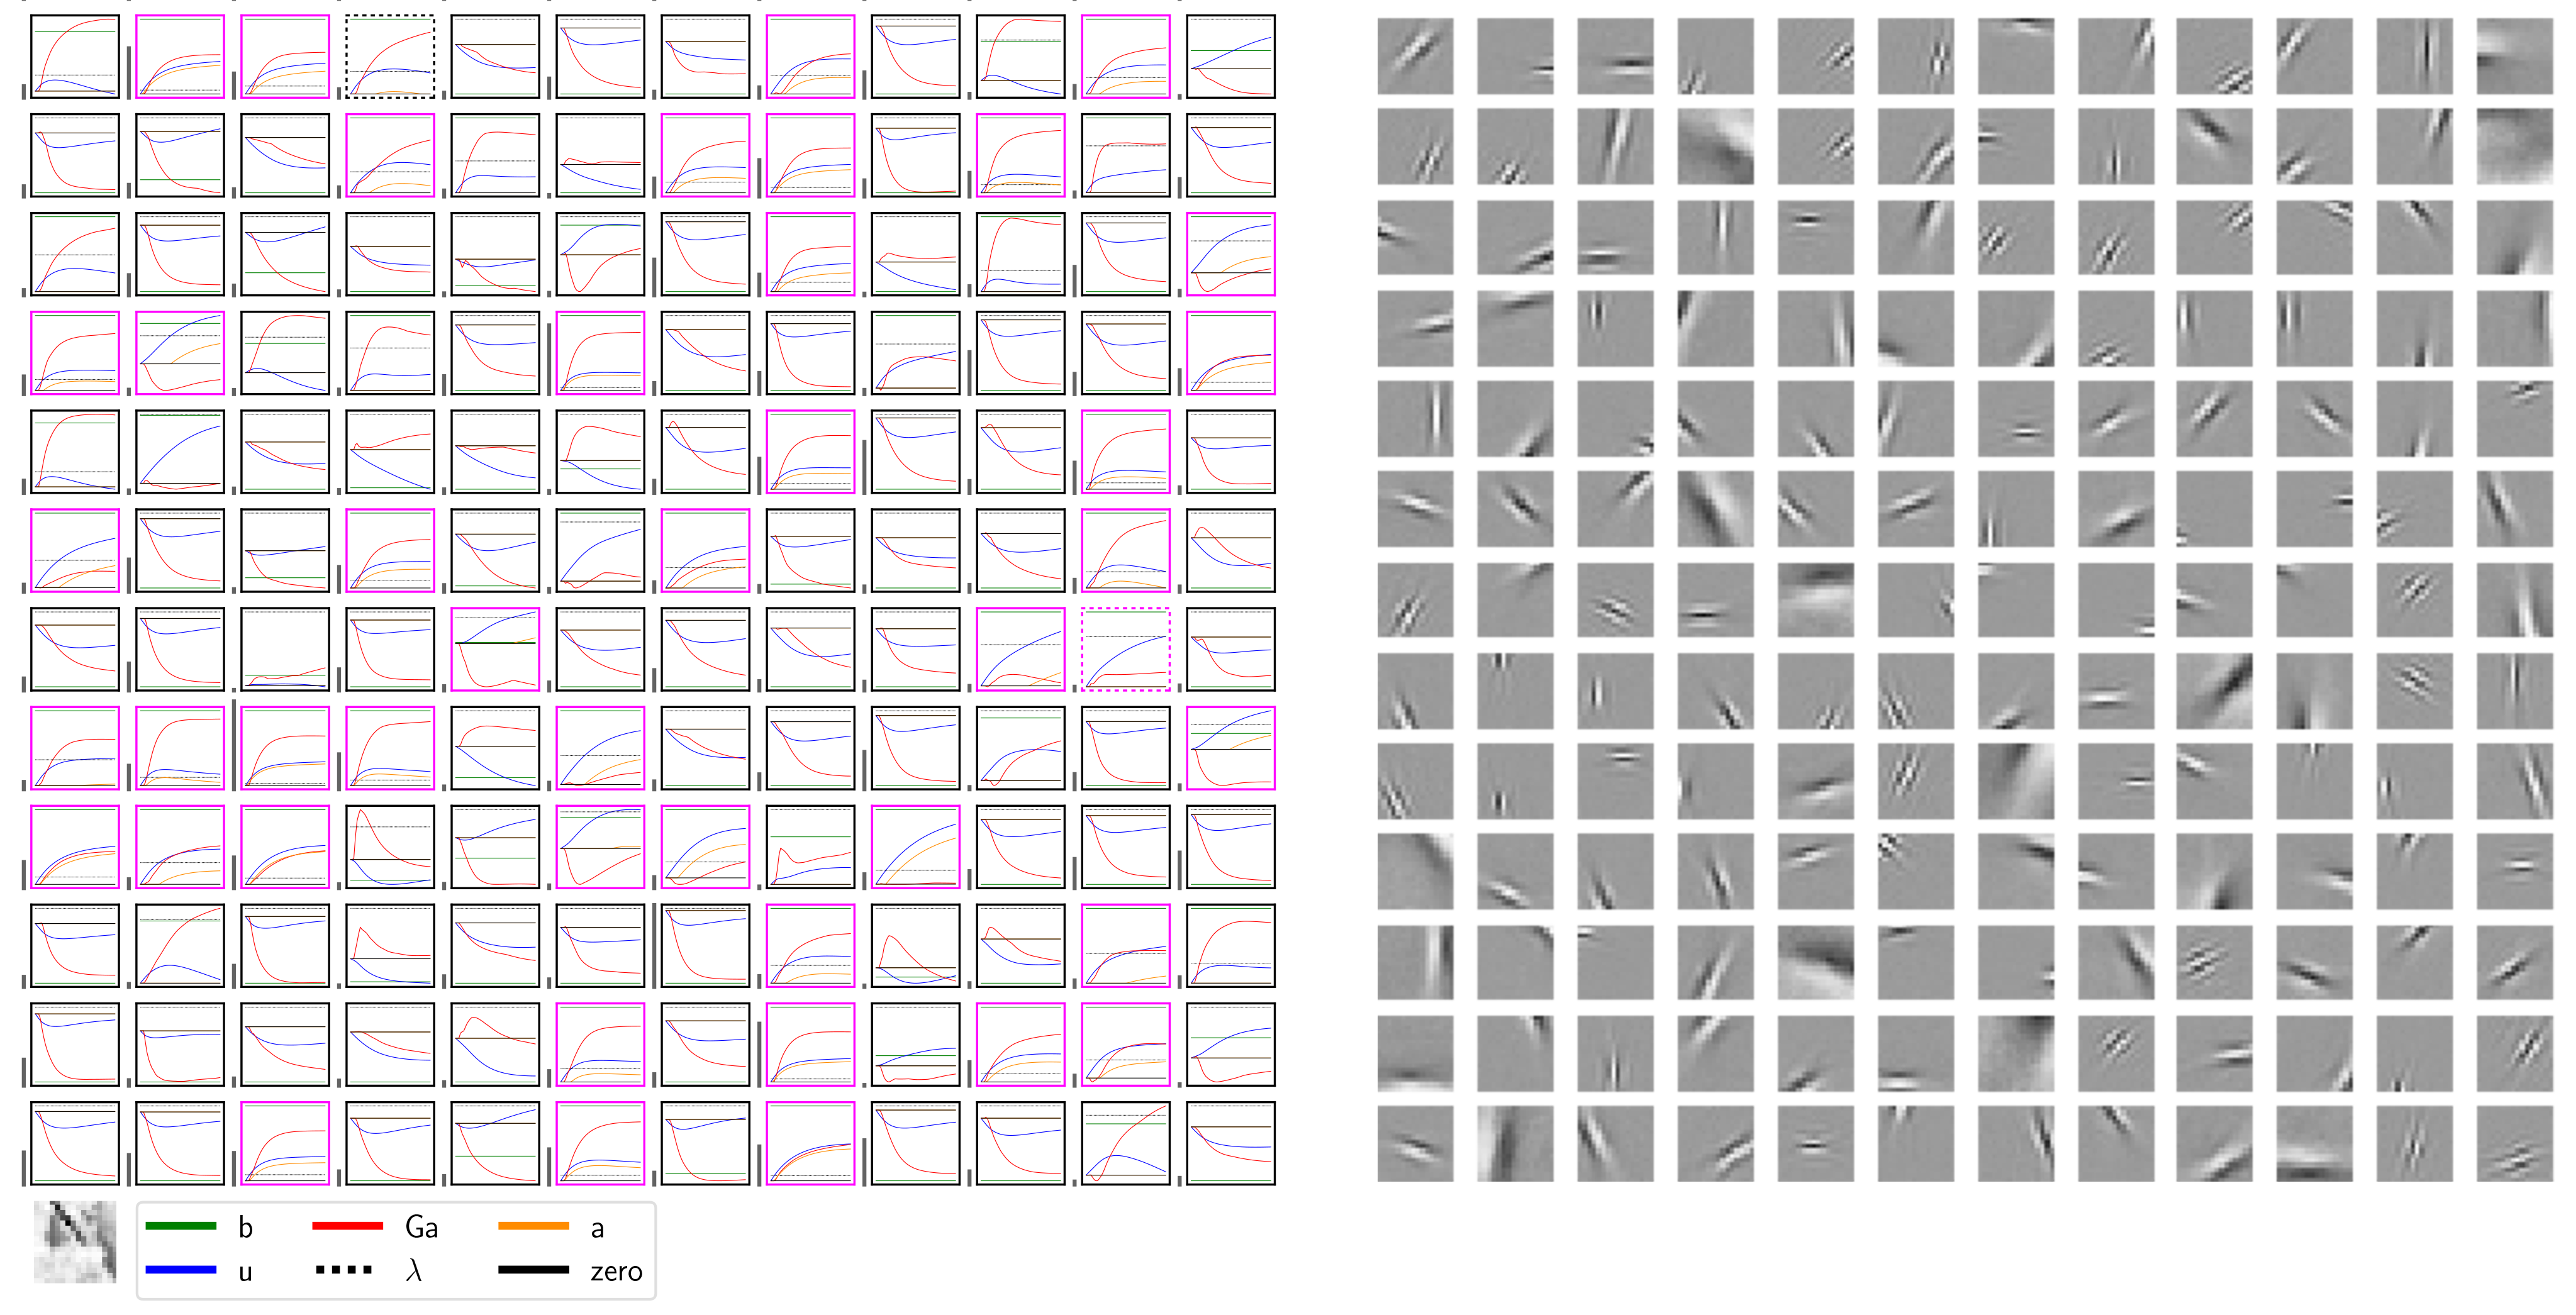
\includegraphics[width=\textwidth]{figures/lca_inference_traces.png}
    \caption{Individual trace dynamics for LCA neurons. Shown are input and output traces for a subset out of 768 LCA neurons during inference. The input image is in the bottom left, and on the right is the corresponding weight vector for the neurons. Each line represents a term in equation \ref{eq:ch2_lca_deda_simple}. The grey bars on the left of each trace plot indicate relative scale of the vertical axis. A magenta boundary indicates that the neuron was active at the end of the inference period, and a black boundary indicates otherwise. A dotted boundary indicates that it became active or inactive in the last 20 percent of the inference process.}
\end{figure}


\subsection{Hard thresholded LCA has many energy minima}
It is possible to define a variety of valid threshold functions for converging LCA dynamics. The two primary functions considered in \parencite{rozell2008sparse} are termed ``soft'' and ``hard'' thresholds, which approximate solutions to the $l_{1}$ and $l_{0}$ cost functions, respectively. Much of the work herein is focused on the soft threshold function, as described in \ref{eq:ch2_lca_threshold_func}, primarily for model simplicity. However, the hard thresholded variant is highly intriguing as it results in a higher degree of non-linearity and solves a harder optimization problem with many alternate local minima. The rectified hard thresholded LCA model behaves exactly as is described in section \ref{sec:ch2_lca}, except that the thresholding function has been changed to:

\begin{equation}\label{eq:ch2_lca_hard_threshold_func}
    T_{\lambda}(u_{k}(t)) = \left\{
    \begin{aligned}
        0,\;\; &u_{k}(t)\; \leq\; \lambda \\
        u_{k}(t),\;\; &u_{k}(t)\; >\; \lambda
    \end{aligned}
    \right.
\end{equation}

As is described in \parencite{rozell2008sparse}, this variant approximates the $l_0$ cost function for $C(\cdot)$ in equation \ref{eq:ch2_sparse_energy}. Hard thresholded LCA performs similarly to the soft thresholded variant, except that there is no longer a convex energy landscape with a single global minima. After some number of inference steps, the LCA model settles to a stable minima, but in \parencite{shainin2016sampling} we show that the minima reached by a convolutional, rectified, hard thresholded LCA is not a global minima. It is not clear how the amount of information differs between these minima. However, it has been proposed that the brain could represent likely events in a probabilistic framework \cite{lee2003hierarchical} and that sampling could be a mechanism for decoding signals in higher cortical areas \cite{hoyer2003interpreting}.

To better understand the energy landscape, we sampled a number of approximately equivalent minima (in terms of energy) for sparse codes trained on the CIFAR10 dataset \parencite{krizhevsky2009learning}. We performed this sampling by allowing the network to settle to a minima for a given image, then perturbing the neuron activations with Gaussian noise, and allowing it to settle again. We measured the distances between fixed points by counting the number of neurons that changed their activity, which is equivalent to the Hamming distance between binarized (changed or didn't change) vectors. Figure \ref{fig:ch2_lca_fixed_point_distances} shows that the Hamming distance from the original fixed point to the perturbed fixed point grows as we continue to perturb the network until it reaches a plateau. The figure also shows that the network \textit{always} settles on a different minima.

\begin{figure}[h]\label{fig:ch2_lca_fixed_point_distances}
    \centering
    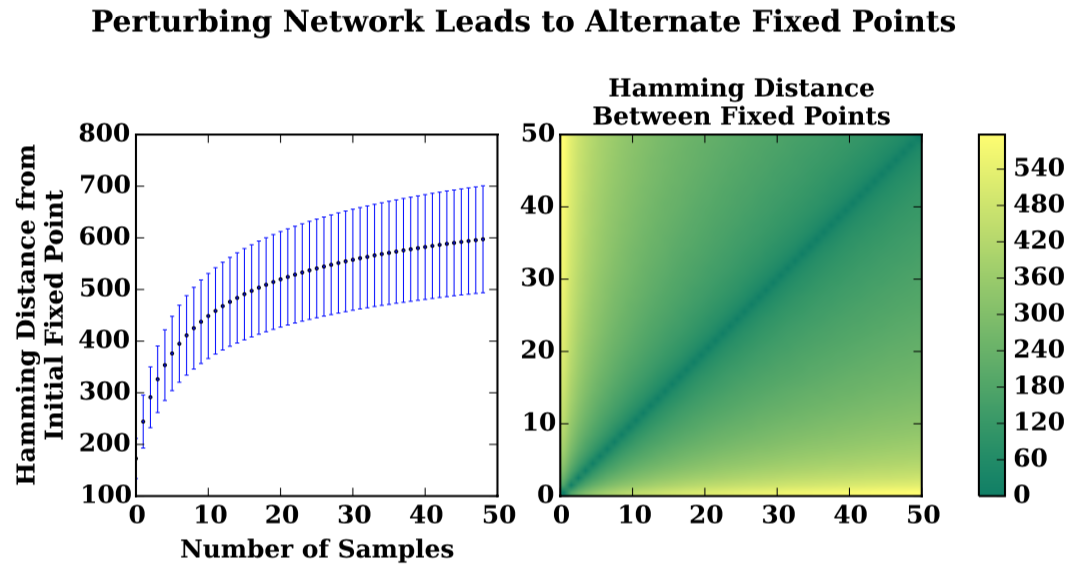
\includegraphics[width=075\textwidth]{figures/lca_fixed_point_distances.png}
    \caption{The hard thresholded LCA model has a number of valid fixed points in terms of the energy defined in equation \ref{eq:ch2_sparse_energy}. If you allow the model to settle to a minima, then perturb the latent code with Gaussian noise, it settles to a different location. Left: The Hamming distance between codes from the original fixed point to the perturbed fixed point after many perturbations. Hamming distance is measured by assessing how many neurons changed their activity value. Right: Hamming distances between all pairs of fixed points for all perturbations. Note that all values are above 0, which indicates that the model always settled to a unique minima after perturbation. This figure was reproduced with permission from \parnecite{shainin2016sampling}.}
\end{figure}

In figure \ref{fig:ch2_lca_norms_and_acc}, we show that the $l_{0}$ sparsity of the activations improves as we continue to perturb the input while the reconstruction error remains the same, suggesting that it is finding better minima. To understand the information content of these minima, we trained two layer classifiers on the sparse codes produced after convergence. The first experiment was to average the fixed point vectors together. We show that the classification accuracy increases as we add more fixed points to the average, which implies that there is different information content per fixed point. The second experiment was to search the independent fixed points for whichever produced the highest confidence (in terms of minimum entropy of the classifier's output distribution) and use this single fixed point as input to the network. The right panel in figure \ref{fig:ch2_lca_norms_and_acc} shows that the classifier accuracy improves as we increase the number of candidates in the search. Additionally, we found that the number of perturbations to achieve a fixed point with highest confidence was highly variable (not shown).

\begin{figure}[h]\label{fig:ch2_lca_norms_and_acc}
    \centering
    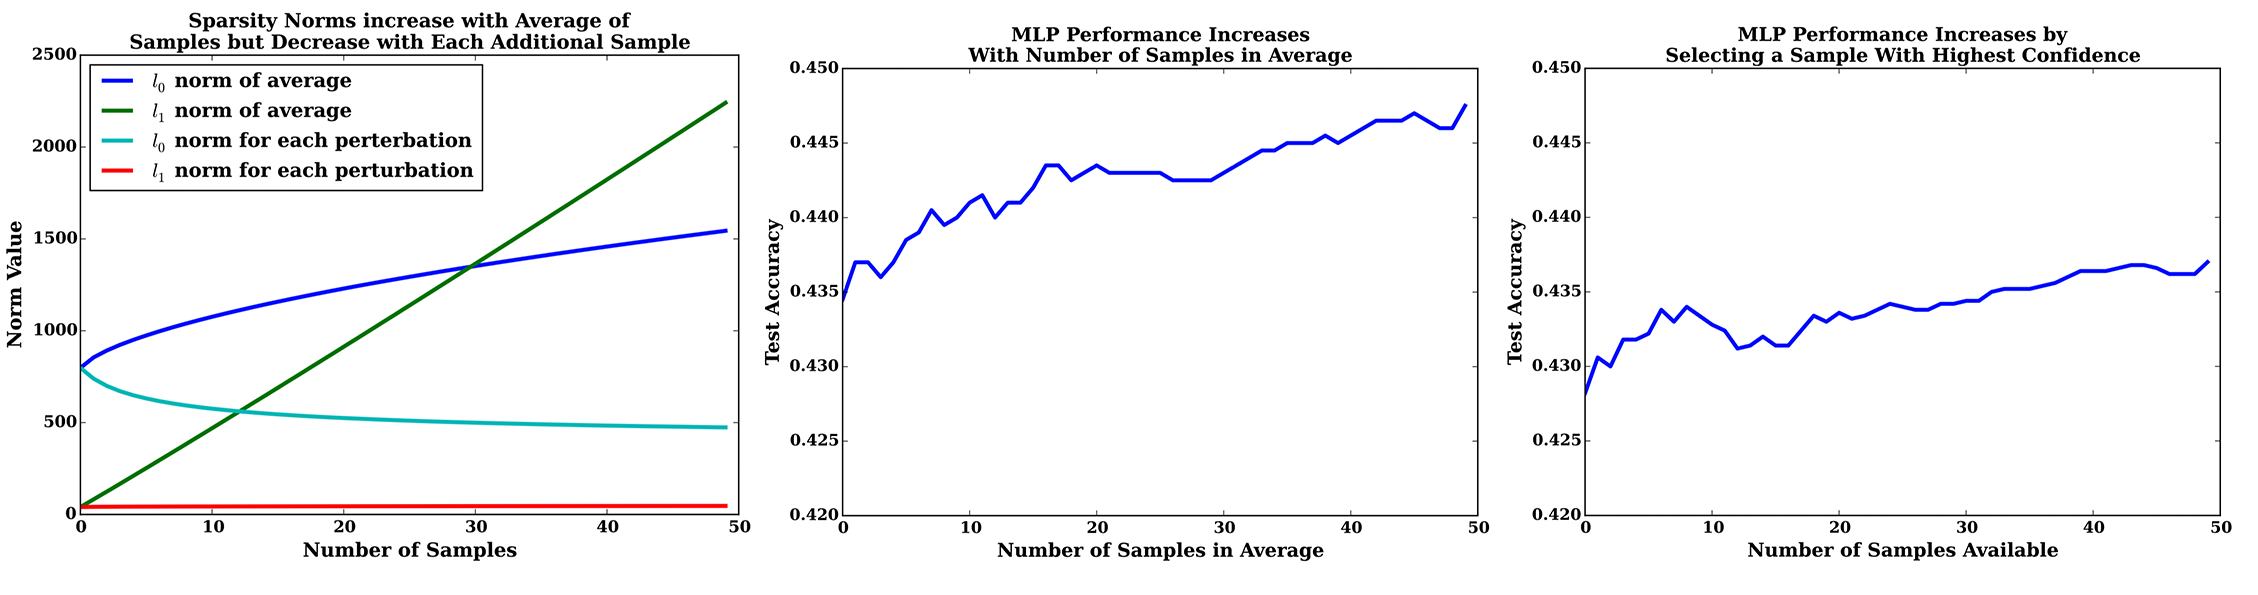
\includegraphics[width=\textwidth]{figures/lca_norms_acc.png}
    \caption{Fixed points have different sparsity and contribute unique information for a classification task. Left: New fixed points after perturbing the hard thresholded LCA network tend to have better $l_{0}$ norm. The dark blue and green lines show that norms increase when we average together the codes from each perturbation, which is to be expected. The cyan and red curves show that as we continue to perturb the activations, the network settles on a minima with approximately equal $l_{1}$ norm and an improved $l_{0}$ norm. Middle: We construct an averaged vector from each fixed point and use that as input to a classifier network. The classifier accuracy improves as the number of vectors in the average grows, indicating there is additional information in the alternate fixed points. Right: Instead of averaging the fixed points, we search them to determine which one produces a minimum entropy output from the classifier. This fixed point is then used to determine the class label. The figure shows that as you increase the number of samples that are searched over, the classifier accuracy improves. This figure was reproduced with permission from \parencite{shainin2016sampling}.}
\end{figure}


\section{Alternative image coding models}\label{sec:ch2_alternative_image_coding_models}

% TODO:
%\subsection{The linear / non-linear neuron model}
%Simoncelli, etc. Adding components.
%
%
%\subsection{Autoencoders}
%Autoencoders as a NN implementation of L/NL neurons.


\subsection{Predictive coding}
Here we will draw comparisons between the sparse coding model, as described in Olshausen and Field \citeyearpar{olshausen1997sparse} and the predictive coding model described in Rao and Ballard \citeyearpar{rao1999predictive}. The sparse coding encoder is a single layer predictive coding encoder with a linear synthesis function. This is made intuitive by comparing the LCA model, a variant of the sparse coding model, against the predictive coding model.

The objective of this investigation is to explore the encoding processes for sparse coding and predictive coding assuming that we are given a trained dictionary. In our sparse coding energy function (equation \eqref{eq:ch2_sparse_energy}), we use $\lambda$ as a trade-off penalty between the reconstruction quality and the sparsity constraint. In practice we tune it to maximize network sparsity for a minimum accepted reconstruction quality. In Olshausen and Field, \citeyearpar{olshausen1997sparse}, their choice of cost function, $C(.)$, specified a Cauchy distribution for the prior on $a$:

\begin{equation}\label{eq:ch2_cauchy_cost}
  C(a_{i}) = log(1+a_{i}^{2})
\end{equation}

For a learned dictionary, to encode an input image we compute a coefficient vector, $a$. Our coefficients (neuron activations) adapt to minimize the energy function described in equation \eqref{eq:ch2_sparse_energy}. The standard way to do this is to perform direct gradient descent on the energy function, following equation \eqref{eq:ch2_lca_deda_extended}, which we will rewrite here with a small algebraic change:

\begin{equation}\label{eq:ch2_sc_deda_rewrite}
    - \frac{\partial E(t)}{\partial a_{k}(t)}
    =
        \sum\limits_{i}^{N} \Phi_{i,k} \left(S_{i} - \sum\limits_{j}^{M}a_{j}(t) \Phi_{i,j}\right) -
        \lambda \sum\limits_{j}^{M}\frac{\partial C(a_{j}(t))}{\partial a_{k}(t)}
\end{equation}

A block diagram illustration of this encoding process is given in \ref{fig:ch2_lca_pc_comp}.

Much like the sparse coding model, the predictive coding model, as described in \parencite{rao1997dynamic, rao1999predictive}, is a neural network that aims to implement efficient coding for natural visual stimuli. Although the predictive coding model is described in a more general fashion, the actual implementation used for experiments ends up being strikingly similar to the sparse coding model. Assuming a learned dictionary, the energy equation for the predictive coding model is as follows:

\begin{equation}\label{eq:ch2_pc_energy_func}
        E =
        \tfrac{1}{\sigma_{S}^{2}} \|S - \hat{S} \|_{2}^{2} +
        \tfrac{1}{\sigma_{td}^{2}} \|a - a^{td}\|_{2}^{2} +
        \lambda \sum\limits_{i}^{M}C(a_{i}),
\end{equation}

where $a^{td} = f\left(\Phi^{1T}a^{1}\right)$ represents the top-down feedback and $\sigma_{td}^2$ is the expected Gaussian variance of the $a^{0}$ estimate. As they describe it, this is a combination of the ``sum of squared prediction errors for level 1 and level 2, each term being weighted by the respective inverse variances.'' The energy function also includes a cost on the activations, which for this example will still be derived from the Cauchy prior. A key difference here between this model and the sparse coding model is how the image approximation, $\hat{S}$ is computed. Rao and Ballard describe a non-linear synthesis function, $f(.)$, which is used in the reconstruction:

\begin{equation}\label{eq:ch2_pc_synthesis}
 \hat{S} = \sum\limits_{i}^{M}f(\phi_{i}a_{i})
\end{equation}

If $f(.)$ is the identity function (i.e. $f(x)=x$), then we get the sparse coding reconstruction energy term. Rao and Ballard describe this as a ``lateral inhibition'' model, although the form of synthesis should not actually differentiate between a feedback or lateral inhibition model. In their study, they experiment with both an identity synthesis function and a $tanh(.)$ synthesis function.

Again we can take the derivative of equation \eqref{eq:ch2_pc_energy_func} to get our update rule. In \parencite{rao1999predictive} they include a time constant for the iterative update procedure, which we will leave out for clarity.

\begin{equation}\label{eq:ch2_pc_deda}
    - \frac{1}{2}\frac{\partial E}{\partial a_{k}}
    =
        &\frac{1}{\sigma_{S}^{2}}\sum\limits_{i}^{N} \Phi_{i,k} \left(S_{i} - \sum\limits_{j}^{M}a_{j} \Phi_{i,j}\right) -
        \frac{1}{\sigma_{td}^{2}}\sum\limits_{i}^{M}(a_{i}-a_{i}^{td}) -
        \lambda \sum\limits_{j}^{M}\frac{\partial C(a_{j})}{\partial a_{k}}
\end{equation}

Comparing equations \eqref{eq:ch2_pc_deda} and \eqref{eq:ch2_sc_deda_rewrite}, one can conclude that the two differences between the predictive coding model and sparse coding model is the (potential) use of a non-linear synthesis function and a second layer of processing. This is illustrated pictorially in figure \ref{fig:ch2_lca_pc_comp}.

\begin{figure}[h]\label{fig:ch2_lca_pc_comp}
\centering
    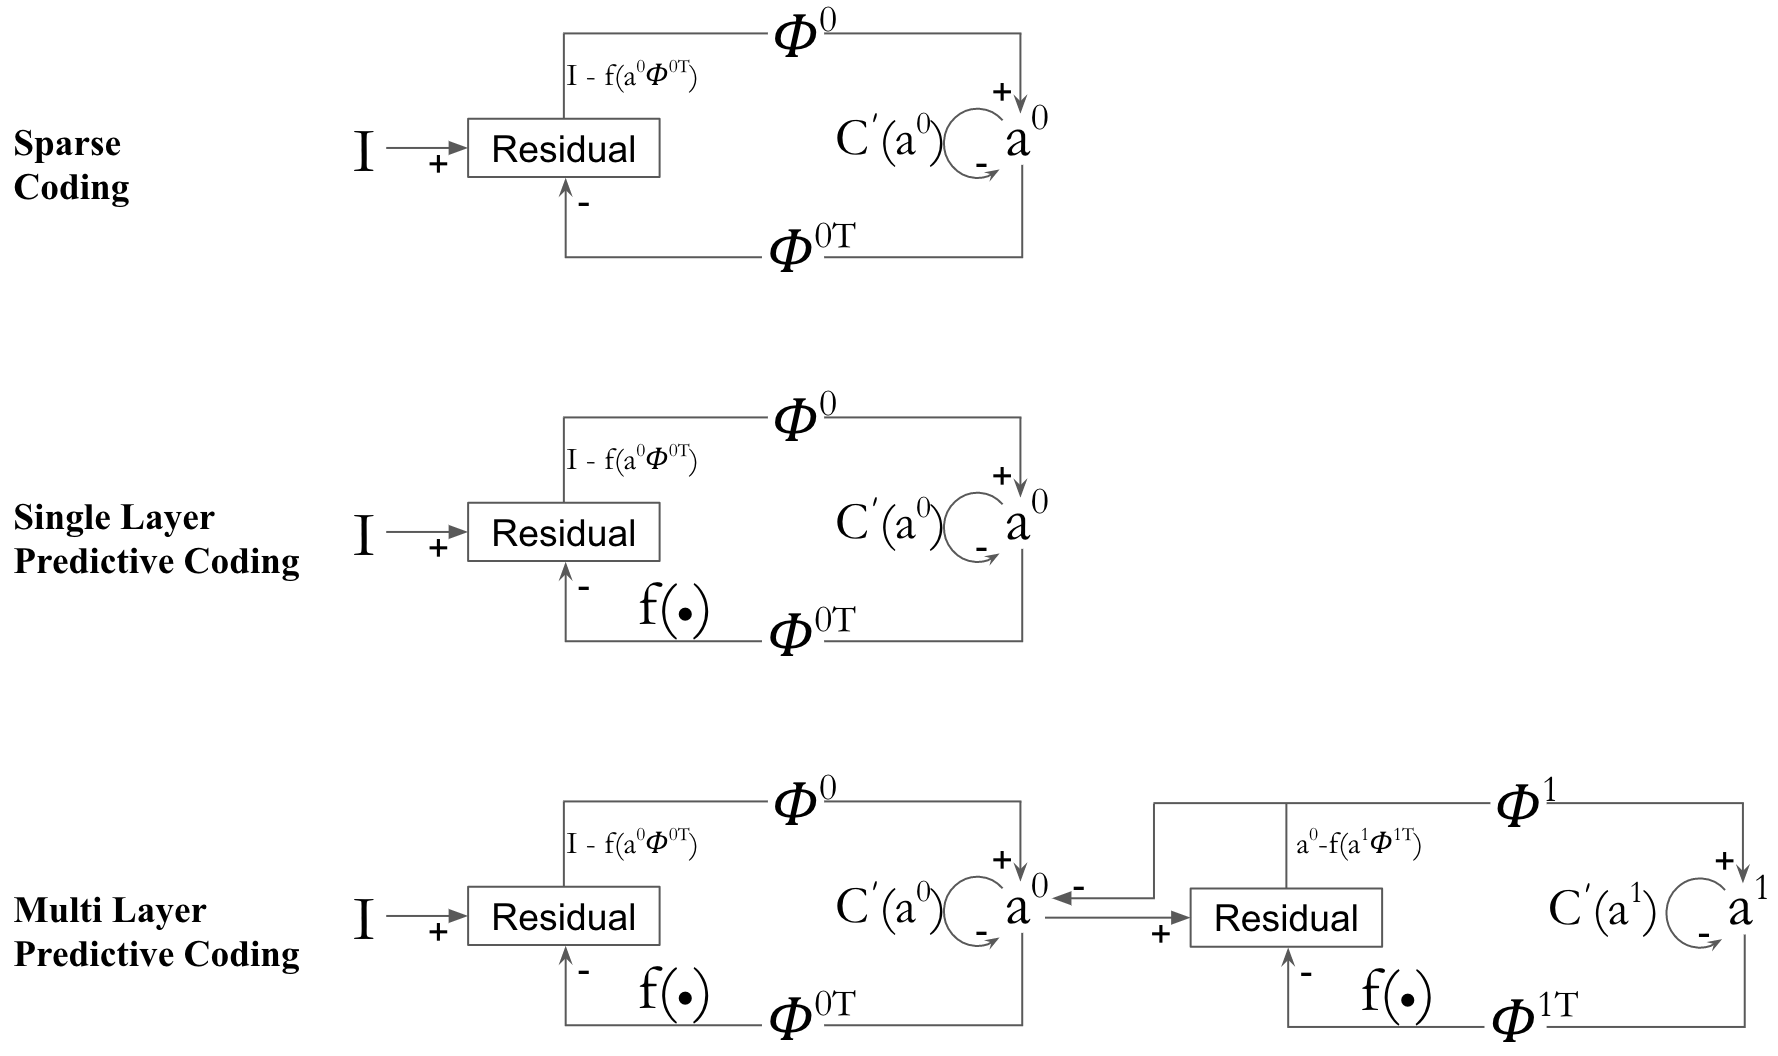
\includegraphics[width=\textwidth]{./figures/lca_pc_model_comparisons.png}
    \caption{\textbf{Model Comparisons} Sparse approximation can be performed via direct gradient descent on the energy function (Equation \ref{scenergyfunc}). This can be thought of as a dynamic process, as depicted here. Adding a non-linearity to the synthesis function results in a single layer of the predictive coding model. The full model, as described in \cite{rao1999predictive}, combines two such layers.}
\end{figure}


% TODO:
%\subsection{Iterative Subtraction as a Form of Divisive Normalization} \label{divnorm}
%In their nature publication \cite{rao1999predictive}, Rao \& Ballard suggest that repetitive subtraction of neighboring neuronal activities may produce a net effect similar to divisive normalization. Eero's group has look extensively into divisive normalization - this section is intended to attempt to draw a link between the two.


\subsection{ICA}
Sparse coding and ICA are related algorithms that employ similar linear generative models, but differ critically in their encoding processes. The image code produced by ICA is computed linearly, whereas sparse coding computes the code with a nonlinear inference process. Here we show that this nonlinear encoding process confers a considerable advantage in coding efficiency and orientation selectivity.

ICA assumes the generative model:

\begin{equation}
\mathbf{s} = \mathbf{\Phi a}
\end{equation}

where $\mathbf{s}$ is an image, $\mathbf{\Phi}$ is a matrix of filters and $\mathbf{a}$ is a vector of activations that represents the neural code \parencite{bell1997independent}. The goal of ICA is to learn a set of statistically independent filters such that the input data can be reconstructed with minimal error. In ICA, the filter matrix is square and full rank and thus invertible. This allows the ICA activations for a given input to be computed directly as:

\begin{equation}
\mathbf{\hat{a}} = \mathbf{\Phi}^{-1}\mathbf{s}
\end{equation}

During inference, activations are computed with a single, linear, feed-forward operation. The filter matrix is learned via a non-linear, iterative optimization process to accurately reconstruct the input while maximizing the statistical independence of the filters as measured by the joint entropy of the activations. This process results in filters that are optimized for the higher-order statistical structure in natural scenes.

Sparse coding, however, has a highly non-linear encoding process. The overall optimization procedure involves a fast inner loop in which the coefficients are computed for each data vector and a slower outer loop in which the basis functions are adapted to the statistics of the entire dataset. In the inner loop, coefficients are computed considering the prior on their expected distribution. In ICA, however, the prior plays no role in determining the coefficients, but it does still play an important role in the learning the basis functions.

The ICA learning algorithm is simpler and faster than the sparse coding algorithm because the encoding can be computed from the data in a single feedforward pass. The basis functions are then learned by computing the cost on the code directly. The independent component analysis algorithm of Bell and Sejnowski \citeyearpar{bell1997independent} is formally equivalent to maximum likelihood in the case of no noise and a square system (the dimensionality of the output is equal to the dimensionality of the input). It is easy to generalize this to the case when the number of outputs is less than the number of inputs, but not the other way around. When the number of outputs is greater than the effective dimensionality of the input of non zero eigenvalues of the input covariance matrix then the extra dimensions of the output will simply drop out \parencite{livezey2016degeneracy, le2011ica}. While this does not pose a problem for blind separation problems where the number of independent sources is less than or equal to the number of mixed signals, it will become a concern in the representation of images, where overcompleteness is a desirable feature \parencite{simoncelli1991shiftable}. The main difference between the Olshausen and Field \citeyearpar{olshausen1996emergence} sparse coding model and the ICA algorithm of Bell and Sejnowski \citeyearpar{bell1997independent} is in the simplifying assumptions they make in order to deal with the intractable integration problem posed by finding the set of basis functions that maximize the likelihood of the inputs given the model defined by those basis functions. Olshausen and Field’s algorithm assumes low-noise and thus a peaky, unimodal distribution on the joint probability between the image and the sparse code given the model in order to justify evaluating it at the maximum (MLE), whereas Bell and Sejnowski limit the dimensionality of the code to equal the dimensionality of the input and also assume no noise so that the integral becomes tractable.
